\documentclass[10pt,twocolumn]{article}

% use the oxycomps style file
\usepackage{oxycomps}
\usepackage{hyperref}

% usage: \fixme[comments describing issue]{text to be fixed}
% define \fixme as not doing anything special
\newcommand{\fixme}[2][]{#2}
% overwrite it so it shows up as red
\renewcommand{\fixme}[2][]{\textcolor{red}{#2}}
% overwrite it again so related text shows as footnotes
%\renewcommand{\fixme}[2][]{\textcolor{red}{#2\footnote{#1}}}

% read references.bib for the bibtex data
\bibliography{references}

% include metadata in the generated pdf file
\pdfinfo{
    /Title (Comps Proposal)
    /Author (Justin Li)
}

% set the title and author information
\title{Random Generation For Hack-and-Slash Roguelike Level Templates}
\author{Lukas Howlett}
\affiliation{Occidental College}
\email{lhowlett@oxy.edu}

\begin{document}

\maketitle

\section{Introduction and Problem Context}

An established practice of game developers working on roguelike video games is to utilize random level generation in lieu of creating each level manually by hand. By generating levels randomly, the developers are able to increase replayability of the game since players will never encounter the same level layout twice. This coupled with another feature of roguelikes called "perma-death", where the player loses all progress upon dying, makes for great game design as players will often end up losing and restarting due to the higher than average difficulty of roguelikes; but because the layout of the levels change upon each playthrough of the game, gameplay stays fresh as the player will encounter unique scenarios that they may not have seen in their last playthrough.

Moreover, with the rising popularity of roguelikes in modern game-development such as \textit{Hades}\cite{hades} and \textit{Dead Cells}\cite{deadcells}, the need for interesting random level generation designs rises as well. The goal of this project is to create a random level generator in the Unity game engine that game developers can use to create level templates with difficulty progression for a fast-paced, "hack-and-slash" themed, roguelike game. The relevance of this project is that it can be used as a tool to help game developers/coders create their own roguelike levels without needing to leave the Unity editor software. The reason for why this is important is because some developers/coders lack the technical skills to be able to produce a random level generator of their own, meaning that with this project they can focus on other aspects of development instead. Ultimately, this will serve to bridge the skill-gap between lesser and more skilled game developers, allowing less-skilled developers to catch up to more-skilled developers who can already develop their own random level generators. 

\section{Technical Background}

\subsection{Unity Terminology}

Since this project is based around game-development, this paper will define and use many technical terms originating from both computer science and video games as well as the gaming community itself. The most relevant of which that hasn't already been defined is the platform in which this project is created, the Unity Game engine and game engines themselves. Game engines are software frameworks that are primarily designed to create and develop video games and typically include supporting programs such as a level editor\cite{valencia2016technologies}. The Unity game engine has such a level editor in which a developer can add gameobjects, which represent fundamental objects in Unity such as characters, props, and scenery, into the level that they're editing. For projects that utilize matrices for level design, like this one, Unity offers a Tilemap package which includes a grid and tilemap gameobject; the grid acts as a canvas for the tilemap which holds an assortment of tiles(sprites), which are 2-dimensional graphical objects, that can be "painted" onto the grid to form levels. 

In order to manipulate gameobjects in Unity, scripts must be added onto them. Therefore the only way to paint tiles onto a grid randomly, is to create a script that can select specific tiles and place them onto the grid on its own. Technically, this project works by utilizing Unity's tilemap package, adding a custom script onto another gameobject, and then creating functionality between the script and Unity level editor from within the script. 

\subsection{Game Terminology}

Roguelikes, which were previously mentioned but never officially defined, are a sub-genre of video game that are categorized by random level generation and perma-death of the character. Other technical video game terms include mechanics and gameplay. Game mechanics are the underlying rules of a video game that ultimately decides how players will play the game\cite{boller2013learning}. On the other hand, gameplay is the combination of many elements within the game such as difficulty, enemies, level layout, and how the player can interact with them using the game's mechanics\cite{tyler2023what}.

This project aims to create level templates which fit "Hack-and-Slash" gameplay, which is a type of gameplay defined by quick, close range combat with melee or close-range weapons and often includes versatile player movement such as a dash mechanic that allows the player to move really quickly in small bursts of speed. \textit{Hades} and \textit{Dead Cells} are both classified as hack-and-slash games as they both provide a broad range of melee weapons for the player to use as well as a dash or other types of movement mechanics. Additionally, difficulty progression is the gradual increase in difficulty the further a player progresses within the game. In \textit{Enter the Gungeon}\cite{enterthegungeon}, difficulty progression can easily be identified by comparing the starting levels to the endgame levels; the starting levels are very simple including maybe 3-4 of the same enemy with very little hit-points(HP), which is the amount of life an enemy has, whereas the endgame levels are much more complex including many different types of enemies and environmental hazards/traps. The level templates created by this project attempt to create this difficulty progression, or at least give the player a sense of one, as they progress. 

Because it is relevant to the harsh difficulty often associated with roguelike games, one last term that needs to be defined is glass-cannon. In games, glass-cannons are typically an enemy or character-type that features high damage output in combination with low HP. Therefore glass-canons are able to kill enemies or players in a short amount of time and are balanced out by the fact that they too can be killed in a short amount of time. This project assumes that the playable character would be a glass cannon and takes that, as well as difficulty progression, into account when designing levels.

\section{Prior Work}

\subsection{"Hack-and-Slash" Roguelikes}

As was mentioned earlier in the paper, this project aims to design level templates based around hack-and-slash gameplay; many different games have already been created with this type of gameplay, so this paper will focus specifically on other roguelikes that are also hack-and-slashes. 

In both \textit{Hades}\cite{hades} and \textit{Dead Cells}\cite{deadcells}, the player can choose from one of many melee weapons and has the ability to dash around the map, defining them as a proper hack-and-slash games. Each game also offers fast gameplay with glass-cannon characters that can utilize abilities to move around the room and map at exceptional speeds. While similar in many aspects, a big difference between the two is that \textit{Hades} features a more traditional roguelike 2D top-down gameplay perspective whereas \textit{Dead Cells} features a side-scrolling gameplay perspective which is usually more typical of platforming games. Because their gameplay perspectives are not the same, many other differences also become apparent as a result. For example, in \textit{Dead Cells} the player has the ability to jump which makes sense for a side-scroller's perspective, but from a 2D top-down perspective like in \textit{Hades}, jumping wouldn't make sense since the player views the player from the top-down and wouldn't be able to see their character jump. Overall, this difference in gameplay perspective shows that there are noticeable variations in game design between 2D top-down hack-and-slash roguelikes and side-scrolling roguelikes as a result of what mechanics make sense for each perspective.

I brought this to attention because this project aims to generate levels for 2D top-down hack-and-slash roguelikes. This means that certain aspects of game and level design that may make sense for \textit{Dead Cells} wouldn't make sense for my level generator. The aspects of \textit{Dead Cells} that do make sense for my level generator however, such as topographical and combinational spawns, were taken into account. 

\subsection{Topographical Spawns}

When an enemy is spawned, meaning generated within the map, at or near certain topographical points in the level, that is a topographical spawn. This is done to give the generated levels some character and the player a sense of what to expect when coming across these landmarks in the map. This can be seen in \textit{Dead Cells} when the player is able to make it to a level called "The Bank"; there are piles of gold scattered throughout the map and sometimes an enemy called the 'agitated pickpocket' will spawn next to them or in areas close to them. \textit{Enter the Gungeon}\cite{enterthegungeon} also utilizes topographical spawns as seen with an enemy called the 'mimic' which has a chance to replace treasure chests in treasure rooms and fool the player. What both \textit{Dead Cells} and \textit{Enter the Gungeon} hope to accomplish with these types of enemy spawns is to keep the player engaged and wary of potential threats. By doing this, the game keeps the player's attention as they are always on the look out for certain visual cues/scenery to make sure they're ready for what could be a potential enemy. Another good showcase of topographical spawning rules is \textit{Procgen Arcana}\cite{procgenarcana} which is an online random map generator for medieval towns created by GitHub user Watabou. Despite the fact that \textit{Procgen Arcana} is not a video game, it uses topographical rules in order to generate its maps so that each generated map will look unique while still having all the elements of a medieval town (eg. small houses outside castle walls and larger houses within). 

Although this project is not going to be a full-on release of a digital game prototype itself, it still utilizes topographical spawning rules in order to keep the players attention and add a different type of element to their gameplay. Using topographical spawning rules will also help to ensure that all generated levels will retain individuality from one another while keeping up the appearance of a hack-and-slash roguelike map. 

\subsection{Combinational Spawns}

Whereas topographical spawns are about enemies spawning at or near certain topographical locations, combinational spawns are about combinations of different types of enemies spawning together. Developers do this in order to create different types of gameplay situations for the player to experience; because the level generation is random in roguelikes, combinational spawns are abundant especially when there are many different enemy types. A common example of a combinational spawn would be to have ranged enemies spawn behind melee enemies as this creates a predicament for the player: should they dash pass the melee enemies, risking damage, and deal with the ranged enemy or should they deal with the melee enemies first, risking ranged attacks? Of course these decisions all change from game to game as there are various ways of dealing with enemies in different games. Combinational spawns are found in most roguelikes, so this paper will talk mostly about the ones found in \textit{Diablo IV}\cite{diablo} and \textit{The Binding of Isaac}\cite{thebindingofisaac} to narrow it down. 

Although \textit{Diablo IV} is not a roguelike, it still shares the elements of a top-down hack-and-slash and one of the most common combinational spawns in the game, is that of a 'bloated corpsefiend' next to a large group of enemies with low HP. This makes for a really fun gameplay experience since one of the attributes of the corpsefiend is to explode when the player kills them. Therefore players are incentivized to target the corpsefiend first so that the resulting explosion could possibly result in a satisfying multi-kill and rewarding gameplay. 

\textit{The Binding of Isaac} uses combinational spawns in a more generalized way since the game was created quite a while ago and has simpler underlying mechanics. In game there are two main enemy types, chasers, who chase the player around the map, and aimless walkers, who, as the name implies, walk aimlessly around the map. This inherently creates three different types of enemy-based gameplay: fighting solely against chasers, fighting solely against aimless walkers, and fighting a combination of the two. Combining this with different environments, player abilities, and even more enemy variations allows \textit{The Binding of Isaac} to host a wide variety of gameplay experiences on each playthrough of the game. 

In order to effectively create a wide variety of gameplay scenarios for players to experience in my level generator, combinational spawns are an integral part of the project. It definitely remains on the simpler side, like \textit{The Binding of Isaac}, since I don't have the funds to create a large-scale title; it's able to generate different enemy types either on their own or in groups opening up avenues for various types of gameplay, despite its simplicity.

\subsection{The Ideal Hack-and-Slash Roguelike}

Having explored the common elements of hack-and-slash roguelikes, this project's vision was set on generating levels for a glass-cannon character using topographical and combinational spawns. Doing this would allow the project to generate levels that could: 1) keep the player engaged, and 2) create various gameplay scenarios so that no two playthroughs would be the same. Therefore, the generated templates retain the common features of a hack-and-slash roguelike while being able to stay unique on each generation of the map. 

\section{Methods}

There were many design decisions made in the process of developing this project which changed or were influenced multiple times as the scope of the project became narrower and more focused; these choices eventually helped mold the project into what it has become now.

\subsection{Unity Game Engine}

For the final build of my project, I ultimately decided to go with the Unity game engine for a number of different reasons. The first of which is that the Unity engine comes with a downloadable Tilemap package which I previously explained in the Technical Background section. This package allows me to easily create 2D top-down environments in Unity's level editor by using tile-based sprites and letting me "paint" them onto the level's grid. There are also a number of useful functions that the Tilemap package has such as grid clearing, checking whether a cell in the grid is holding a tile, and setting/removing tiles from a cell which can all be executed automatically from within a script. Using these functions, I was able to create a script that allowed me to rapidly test my generator by wiping the grid free of tiles and then setting/removing tiles to build an entirely new map with the press of the 'return' key. I could then view these maps from both the scene view, which showed me the entirety of the map, and the game view, which only allowed me to see a smaller section of the map, to see what errors there were and let me know what changes I'd need to make to the generator's code. 

Another reason why I chose to use the Unity engine is because I have a lot of experience working in Unity from both previous courses and personal projects, so I figured working in Unity for my COMPS project would give me the biggest advantage. Also Unity scripting is all done in the C-sharp coding language, which I have built up an extensive knowledge of, therefore choosing Unity for this project became an easy choice. Also worth mentioning is that the Unity editor comes with a 'project' tab that allows developers to sort and organize all of their assets(scripts, sprites, etc.) into organizable sub-tabs. With this knowledge, I knew I'd be able to utilize Unity's inspector tab and scripting system to build functionality between the two and build a useful/easy to use tool for developers. 

Lastly, Unity also has Long Term Support(LTS) for many of its editor versions, meaning that developers using this tool in their projects will have guaranteed support and stability while working on their project so long as they are using a Unity Editor version with LTS. 

\subsection{Level Generation Order}

Level templates were generated by first filling the map with a number of rooms and then generating connecting passageways between those rooms to ensure the entire level is accessible to the player. While the order in which either rooms or pathways are generated first may not seem to matter too much, it was a big decision in the direction of this project as I initially wanted to generate my level templates with the path first and have rooms generate around it. The reason I wanted to generated levels this way was because in game design, especially roguelikes, there's a term called the "critical path" which is the path that hints to the player and tells the computer where the quickest route to the end of the level is\cite{castro2016level}. This is useful as it helps give levels a sense of flow that the player can use to get to the end of the level or ignore if they wish to explore the other sections of the map first; it also helps helps the computer by allowing it to know where the end of the level is meaning it'd be able to generate rooms around it accordingly, keeping the start and end of the level far apart. 

Unfortunately, I eventually had to scrap the critical path idea for time to be able to focus on developing other aspects of the generator's level design such as the topographical and combinational spawning rules, which I'll get into later. Figure 1 below is an image of the generator's path creation algorithm which uses the Unity Engine's random function to act as a basic Random/Drunkard's walk. The Random/Drunkard's walk algorithm works by choosing a random point in the game's map and then moving randomly until the level is completed\cite{koesnaedi2022implementation}. However, I modified this one so that it starts from the left and can only move left, right, or down depending on previous tiles and whether the cell is within the bounds of the grid. 

%INSERT IMAGE OF PATH-FIRST GENERATION HERE
\begin{figure}[h]
\centering
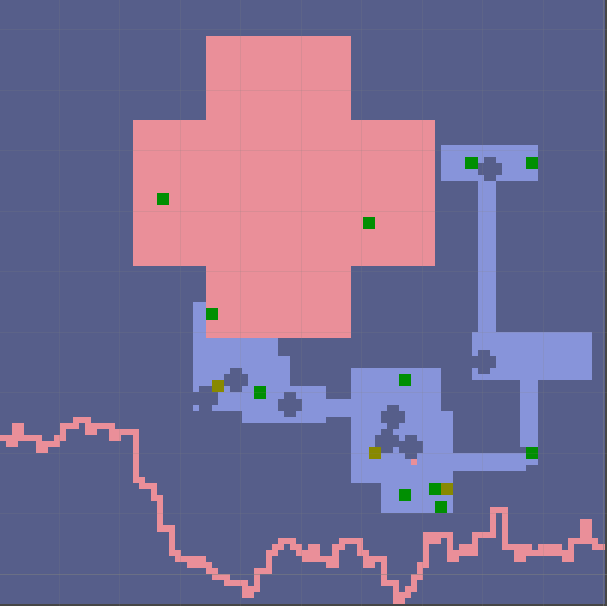
\includegraphics[scale=0.5]{Images/map5.png}
\caption{Path first generation template}
\label{fig:x path first generation}
\end{figure}

The downsides of generating level templates in this order, in terms of this project, were that the generated path seemed to be a little too disconnected with the rest of the map. This had to do with the path generation starting on the left side of the map and ending on the right, leaving the start and end points a little too separated from the other generated rooms. Essentially this made it so that even if I generated pathways between those rooms, the critical path I was attempting to make would occasionally not even be connected to the rest of the level; even when it was connected to the rest of the level, it's value as the critical path wasn't very obvious or had lost its meaning in the other generated pathways entirely. 

Alternatively, creating level templates using room-first generation was a much more simple process and came with tons of advantages that were not shared with path-first generation. Generating the level templates by rooms first allowed me to keep track of each of the rooms' midpoints, which in turn could be used to generate pathways between each of the rooms that flowed from one room into another; so even if the map did not have a well defined critical path, it was able to flow from one section of the map into another in a natural manner. Overall, room-first generation looked much more aesthetic than path-first generation and could create templates that had a natural circulation of pathways. 

\subsection{Map Size, Resizing, and Inspector Attributes}

Each level template is generated on a 100x100 tile grid and fills the level with 'x' amount of rooms that vary in size based on random chance(50x50 being the largest and 5x5 being the smallest). 100x100 was chosen as a baseline grid size for testing purposes, however developers can resize the generated map template's x and y dimensions to their liking from within Unity's insepctor window so long as the selected gameobject has the 'TileMapGrid' script attached to it. Figure 2 below is an image of the TileMapGrid script's attributes from within Unity's inspector tab.

%INSERT IMAGE OF TILEMAPGRID INSPECTOR VIEW HERE
\begin{figure}[h]
\centering
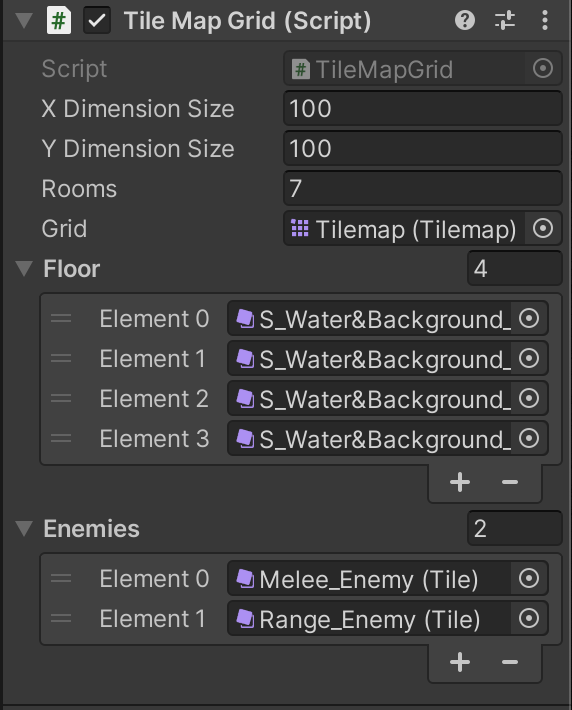
\includegraphics[scale=0.5]{Images/inspector.png}
\caption{TileMapGrid inspector attributes}
\label{fig:x inspector attributes}
\end{figure}

From this image I'd like to observe that there are five modifiable elements that developers can play around with to generate level templates that suit their preferences. The first of which that have already been mentioned are 'X Dimension Size' and 'Y Dimension Size' that both start at a default size of '0' but can be modified to change the overall size of the grid which the level template will be generated upon. Next is the 'Rooms' attribute which controls the the total number of rooms that will be generated within the size of the grid. It should be noted that rooms have a chance to spawn  within, but not completely within, one another as a means to create rooms with different shapes other than square or rectangular; this is done because Unity's tilemaps are unable to easily generate rooms of different shapes. Therefore if the number of rooms does not match what is entered in TileMapGrid's attributes, it is because a room or two have generated within one another. This aspect of the generator should be accounted for when developers choose a number of rooms for the generator to spawn and overall grid size should be considered here as well (the smaller the map, the more likely rooms will generate within another and vice versa). The 'Grid' attribute is simply for the script to be able to reference which grid it will be applying tiles to as there can be multiple grids in a Unity scene. 

Lastly, there are the 'Floor' and 'Enemies' attributes which hold the tile sprites for the script to place onto the grid; developers can insert their own tile sprites into these arrays to take the place of the placeholder sprites which the tool uses by default. At the moment sprites have to be placed at certain index locations in the array for the generator to work properly because the generator works by accessing index location rather than scan for a specific sprite's name. This was done because sprite names vary and are sometimes very similar for organizational purposes meaning it's much easier to just access a specific index in the array.

\subsection{Obstacle and Enemy Spawns}

Obstacle and enemy spawning takes place after the generation of each individual room which places each of the room's tiles into a temporary list for the spawning rules to reference. While scanning through the list of room tiles, the generator is able individually check whether there is enough room to spawn in an obstacle or melee enemy by making tile to tile comparisons as well checking that there is enough space left in the grid. Each room has a chance at spawning any obstacle/enemy combination which are determined by percent chance, location of existing enemies, and topographical location on the map. This is executed by first randomly populating each room with either holes or walls/cover that have a 1/100 chance of spawning on each individual room tile as long as there is enough space to generate one; the same method is used to populate each room with melee enemies. Each obstacle and melee enemy that successfully spawns inside of a room has their spawn coordinates saved to a list that ranged enemy spawns will reference in order to spawn themselves in. Because ranged enemies don't reference each individual room tile for spawning, but rather the spawns of existing obstacles and melee enemies, they have a 1/10 chance of spawning above, below, or on the sides of melee enemies or in the top or bottom corners of obstacles. The reason why ranged enemies only spawn around obstacles or melee enemies is because they require some form of protection from the player whether otherwise it would be far too easy for players to close the distance between them. Additionally, melee enemies have a 1/4 chance of spawning in the corners of corridor pathways from room to room as another form of topographical spawn that will keep players on alert as they travel through these seemingly harmless passageways. 

By spawning obstacles and enemies in this way, the generator is able to showcase the topographical (ranged enemies next to obstscles, melee enemies in corridor corners) and combinational (ranged enemies and melee enemies) spawns that are representative of hack-and-slash roguelike games. This allows the generator to create templates with 9 different types of gameplay including combat against: melee enemies, melee and ranged enemies, melee enemies with cover, melee enemies with holes, melee and ranged enemies with cover, melee and ranged enemies with holes, ranged enemies with cover, ranged enemies with holes, and melee enemies in tight corridor corners. 

Initially, room spawns were going to be determined by assigning each room a difficulty and then spawning in enemies and obstacles according to that room's difficulty. The reason for this was because I wanted to create a sense of difficulty progression for the player and by assigning rooms a designated difficulty, it would guarantee a very linear type of difficulty progression with easy, medium, and hard rooms succeeding one another. However, I ultimately decided against this as I felt that assigning rooms a difficulty in this linear fashion would make the level too tame and predictable. I believed that this type of difficulty progression was too uncharacteristic of the roguelike genre, which is known for its unforgiving nature and higher than average difficulty. Therefore, allowing each room to have a chance at spawning any obstacle/enemy combination made the generated level templates much more unpredictable while still offering the extreme variance in difficulty often seen in roguelikes. 

\subsection{Algorithmic Design}

The random level template generator uses no special algorithms in order to create its levels with the TileMapGrid script being written entirely by myself. The only external source of coding help came from a video by Sunny Valley Studio on YouTube which inspired me to keep track of and connect rooms by saving their midpoints to a list\cite{sunny2021roomfirst}. This helped me especially when I was trying to make passageways between rooms as all I had to do was increase or decrease one room's midpoint coordinates, while simultaneously placing floor tiles, until they finally matched with the xy coordinates of the midpoint of the room I was trying to connect it to. I adapted this to other aspects of my own project as well by saving obstacle and enemy spawn coordinates to their own lists and using them to determine ranged enemy spawns as I mentioned earlier. 

In a way, I believe the TileMapGrid script that I implemented for this project is similar to cellular automata, which is generally an algorithm that revolves around taking an input and then generating a new output based on a developer-established set of rules\cite{minini2020combining}. I think this because each of the tiles in my generator's grid has a chance to change its current tile based on the tiles around it using my predefined rules for level generation. Therefore, my algorithm would be more of a chance-based version of cellular automata where the state of a particular tile is influenced by random percentages and the tiles surrounding it. 

\section{Evaluation Metrics}

Because the scope of my project changed a couple times during its development, the metrics for which it was supposed to be evaluated wasn't set in stone from the start and changed multiple times. Eventually, the final metric for the generator became an evaluation from professor and former game-developer Michael Luo who I worked closely on this project with for his advice and experience in the industry; through many one-on-one meetings with him, he talked about what he wanted to see from my generator. First-off, he wanted my generator to produce levels that are completely accessible to the player, meaning that there should be no areas of the map that the player can't get to. This was a basic requirement which simply meant I needed to make sure that pathways between rooms were never blocked and that all rooms were connected by one path or another. 

Th next things he wanted to see, which is why I've put such a big emphasis on them for this project, were working topographical and combinational spawns. Professor Luo emphasized these in particular in my talks with him as they were essential for creating various types and difficulties of gameplay, especially for hack-and-slash roguelikes. Unfortunately, because I started working closely with Professor Luo closer towards the end of the semester, our talks only included what he'd like to see out of a hack-and-slash level generator and were not able to include what he'd like to see out of the developer tool side of the project. However, the developer tool section of the project was added late in addition to creating the generator and was never part of the project's original scope. To clarify, this project is a random level template generator that models its templates after hack-and-slash roguelike level designs and, in addition to its main function, can also be used as a tool by developers.

Another section of evaluation metric that I want to mention but was not utilized was user-testing of my generator. I asked Professor Luo about potentially using a website called Game Design Reviews\cite{majewski2010game} to obtain additional opinions/suggestions for my template generator, however he said not to as the website was outdated and a review for my project from any online source likely wouldn't be able to happen in a short enough time frame. An additional resource that I also wasn't able to utilize due to time and scheduling constraints, was professor and also former game-developer Scheldon Schiffer who would've been able to offer me another perspective on top of Professor Luo's for what he would've liked to have seen from my template generator. If I had been able to receive advice from Professor Schiffer, I would've been able to consolidate his advice with Professor Luo's and identify what they both found to be essential in hack-and-slash roguelike game design and develop my project with increased focus on their agreed aspects. 

\section{Results and Discussion}

\subsection{Main Results}

The results of the project show that the template generator works well and meets the criterion for what Professor Luo wanted to see from it. Figure 3 below is an image of an example level template created by the generator.

%INSERT IMAGE OF GENERATED TEMPLATE HERE
\begin{figure}[h]
\centering
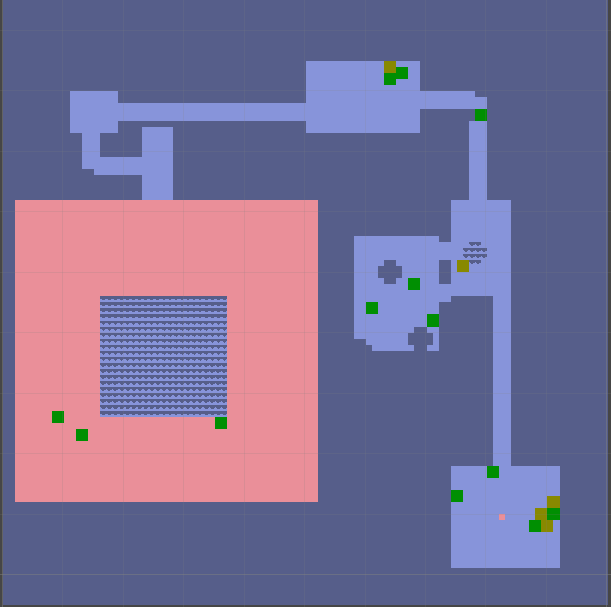
\includegraphics[scale=0.5]{Images/map2.png}
\caption{A complete level template}
\label{fig:x example template 1}
\end{figure}

Because the goal of the project was to generate level templates, the graphics are very basic to act as placeholders for more detailed sprites that I did not have the time to curate or make. The key for this template is as follows: LIGHT BLUE - floor, RED - floor(starting room), DARK BLUE - walls/cover, SPOTTED DARK BLUE - hole, GREEN - melee enemy, YELLOW - ranged enemy. The example template in figure 3 contains all the aspects of level design that Professor Luo required for evaluation metrics. All of the rooms in the generated level are connected and flow from one side of the map to the other. Topographical spawns can be observed in the top right portion of the map where a melee enemy spawns in the corridor's corner and the middle-right portion of the map where a ranged enemy spawns beneath the hole. Combinational spawns can be observed in the bottom right room where there is a cluster of melee and ranged enemies grouped together. Additionally, there is a RED floor tile seen in the bottom right room of the template; while this tile is not part of the starting room, it is there to mark the room with the furthest direct distance from the starting room so as to give an approximate location for where the end of the level should be. 

It should be noted that the generator will not always include each of the 9 types of combat gameplay that it is capable of producing in every generated level because it is all randomized and the types of gameplay will vary from level to level. However, this is by roguelike design since the genre thrives on encountering different types of gameplay on each playthrough of the game. This of course means that sometimes the generator will produce a template that does not include either a topographical or combinational spawn which is perfectly fine as levels would become too monotonous when they're guaranteed to include every single element all of the time. What matters is that the generator has the ability to produce templates including both the topographical and combinational spawns that are essential for this project's evaluation. If I wanted to make every generation uniform with one another I could've, but decided against it to ultimately preserve the inherent random nature of roguelikes. 

\subsection{Takeaways and Alternatives}

Overall, this project had some key takeaways that I believe are worth discussing in more detail for either potential future projects or  beneficial knowledge to have. The first of which is that it was really difficult to create different varieties of room shapes in Unity using the Tilemap scripting system. This is why I eventually decided it was fine if rooms spawned within one another because it would at least give some variety to room shapes. In terms of help or tutorials in scripting different room shapes, I wasn't able to find anything which is one of the biggest downsides of Unity tilemaps for this project; especially because room shapes help communicate to the player certain feelings, with square shapes representing utility, round shapes representing safety and discovery, and sharp shapes representing danger and aggression\cite{plowman2023design}. Therefore being able to utilize various room shapes would've enhanced the players experience by having them learn what shape rooms mean what. Another takeaway that I learned, is that for testing purposes I need tweak the default size of the map and perhaps minimum size of rooms in order to get better overall results. What I mean by this is that sometimes rooms would have spawns that cluttered up the entire room making it look a bit messy. Figure 4 below is an image that shows a template generation with a couple of cluttered rooms on the left and right-most rooms. 

%INSERT IMAGE OF CLUTTERED TEMPLATE HERE
\begin{figure}[h]
\centering
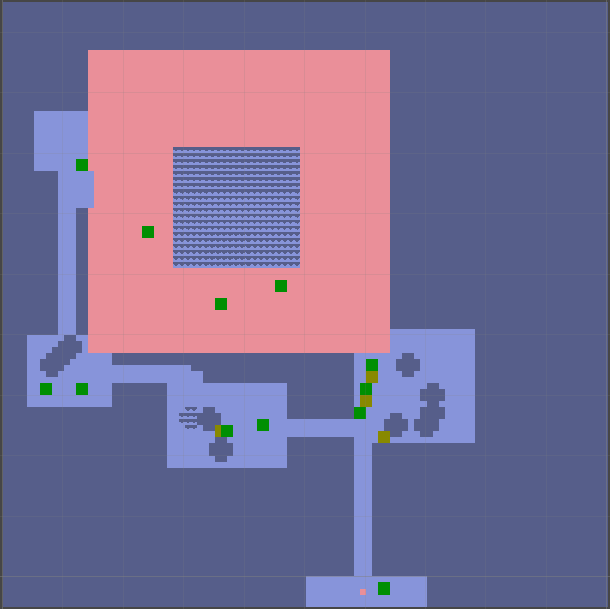
\includegraphics[scale=0.5]{Images/map3.png}
\caption{A level template with cluttered room spawns}
\label{fig:x example template 2}
\end{figure}

Lastly, I think I can definitely enhance my project by adding more obstacle/enemy types as well as figure out a way to include different varieties of room shapes in order to curate more types of gameplay from the generator. Other things that could also add to the possible gameplay experience would be in-game items or even character power-ups. Again this project is merely a level template generator for hack-and-slash roguelikes, leaving lots of creative room for developers who'd like to use it in order to create their levels. 

\subsection{Presentation Feedback}

Among the feedback that I received from both Professors and fellow students during my presentation was that I should consider testing my generator in a playable in-game build, being able to change the spawning rules of different obstacles/enemies from within TileMapGrid's attributes , and have different types of level generations aside from the one I currently have.  By testing my generator in an playable game build, I would be able to get performance results back from my generator outside of Unity's editor environment and therefore reveal to me what flaws my generator would have that would've otherwise not been visible from within the editor. This is important because sometimes the performance of scripts within Unity's editor are vastly different than their performance within an in-game build.

Furthermore, by being able to change the spawning rules of enemies/obstacles, developers won't have to do any work outside of Unity's editor or alter any code. Developers would be able to change, for example, the spawning rules of ranged enemies and have them spawn like how melee enemies do. This way, the generator is a little more flexible as a tool for developers to use so that they'd be able to customize the spawning rules of each obstacle/enemy to their preferences. More spawning rules could also potentially be added; for example, ranged enemies having a chance to spawn in corners or melee enemies spawning next to holes. With this suggestion, it would also make sense for developers to be able to tweak spawn chance of obstacles/enemies to their liking as well.

Lastly, being able to have different types of level generations would certainly add to the variety of possible level generations. However, doing this would require the effort required to build an entirely new generator as the current generator creates levels in its own specific way. Therefore, the only way to include different types of level generations within the same script would be to write an entirely new generator inside said script, which would require far too much time and effort in such a short amount of time. 

\section{Ethical Considerations}

There are a variety of ethical considerations/concerns that arise from my project and since the end result of my project is meant to be used to create video games, common ethical considerations, such as accessibility and violent behavior surrounding video games and video game media, will naturally be intertwined with my work. Also, as mentioned before in the Introduction section, one of the other goals of this project was to serve as a means to bridge the skill-gap between developers of different skill levels. Naturally this means accessibility to game development for those looking to become developers is also discussed. 

\subsection{Video Game Exclusivity/Accessibility}

Although I don't want my project to be exclusive to anyone, the fact that it would contribute towards video game media means that those who are unable to play video games (e.g. disability/accessibility) will unintentionally be excluded. Common examples of people being unable to play because of their disability usually arises due to color-blindness and/or being deaf/hard-of-hearing. While people with color-blindness or hearing deficiencies don't really need to see color or listen to game audio to play video games, it generally keeps them from playing video games properly as both color and game audio are often crucial elements of gameplay mechanics in many video games. Furthermore, people with physical disabilities like cerebral palsy or amputees are also inherently excluded from video games because of an inability to handle a controller or keyboard and mouse. Without being able to input their actions into a controller, playing video games becomes nigh-impossible.

In addition to disabilities, different means of accessibility can also lead to people being excluded from enjoying video games. Whether it's not being able to afford games, not having access to the correct console (platform-exclusive), or living in an area without electricity, there are many different reasons for why someone wouldn't have access to video games. Because of the amount of factors that goes into game accessibility, it's hard to take into account every single one in order to ensure access for everyone.

Keeping those with disabilities in mind, developers using my generator may want to consider disability-inclusive options as an approach. Many modern-day video games try to consider this as well and have introduced options like color-blindness mode, which adjusts game graphics to accommodate for visual impairments, as in the game \textit{Cuphead}\cite{cuphead} or deaf/hard-of-hearing mode, which offers visual and somatosensory cues to assist with  problems of audition, like in \textit{The Last of Us Part II}\cite{lastofus}. Including these options in their games would serve well to include an entire demographic of disabled players, making their games more inclusive and its player-base even larger. In terms of those with physical disabilities, there has been a recent emergence of disability-friendly controllers with tons of customization options to better suit different disabilities. To name a few, there is the Xbox Adaptive Controller \cite{xboxAdaptiveController} which uses a wide variety of switches and buttons to accommodate various disabilities, as well as the 8BitDo Lite SE \cite{8BitDo} which provides easy button-access to low-mobility players, and the Azeron Gaming Keypad \cite{azeron} which is highly-customizable to the point where players only need one hand to play. If developers are able to provide built-in support for these controllers in their games, then they'll be able to be more inclusive of physically disabled players. Furthermore, in order to make their games as accessible as possible, I think making their games free, or at least low-priced like \textit{Hades} which is 25 bucks and still a top-seller, on every available platform would be a great idea. While this doesn't account for every single issue concerning accessibility, it deals with the accessibility issues that are within their control.

\subsection{Violent Behavior}

Because fighting and violence is inherently apart of hack-and-slash roguelikes, I think it's necessary to talk about how violence in video games could possibly perpetuate violent behaviors into the real world. In a journal article by Wadell and Peng, they found that feelings of aggression during a competition can last beyond that initial competitive task\cite{wadell2014does}. However this aggression is not purely the product of video game competition as competition exists everywhere; sports, debates, romance can all evoke feelings of lasting aggression as a result of competition. Moreover, in another journal article posted by Christopher Ferguson, a study was done which found that, "...videogame violence consumption in society [was] inversely related to societal youth violence"\cite{ferguson2015depends}. In other words, the consumption of violent video games by the youth had no correlation to violent crimes committed by that same group of youth. Therefore, violent video games cannot be entirely to blame for violent acts committed by the youth and should be looked upon with a fairer perspective.

In order to prevent the wrong audience from having access to their games and alert parents/guardians of what their games may contain, I would suggest that developers using my generator have their games receive a rating from the Entertainment Software Ratings Board (ESRB) as well as have multiple disclaimers about what content is in their games. The ESRB is an effective tool that both prohibits minors from purchasing games with explicit content and keeps parents/guardians from accidentally purchasing it for them. In a journal article by Laczniak et al., it was stated that, "...parental use of the ESRB might also benefit children by decreasing their exposure to violent images, which should lead to lower overall aggressive behaviors..."\cite{laczniak2017parental}. Because the ESRB has a proven track record of being able to decrease explicit content exposure to minors, I think that developers who use my generator to develop their games should receive a rating from the ESRB to help to ensure that the wrong audience does not find their games.

\subsection{Pathway to Game Development}

In terms of the societal importance of my project, I believe it is very relevant to matters concerning the career path towards becoming a game developer. To put things in perspective, the demographics of game developers in 1989 consisted almost entirely of male game developers with females making up only 3 percent of the game developer population\cite{graser2013videogame}; this also stems beyond gender with a majority 81 percent of the industry consisting of Caucasian  developers in 2019\cite{weststar2019survey}. This is due to the fact that historically, white males were the only demographic with enough money to buy computers and video games; this led to them becoming the only hobbyists in video game development, which eventually gained major popularity, explaining why the industry is so saturated with them today. 

In both the gender and racial minority, a concurring issue that they both have is a lack of relevant knowledge and education concerning STEM courses and video games\cite{ramanan2017issue}. This is why I believe that my project is so relevant to this issue and holds a significant amount of societal importance. While my level generator does not solve the lack of education issue directly, it serves as a workaround for people who lack the knowledge in the first place. This way, even when being used by those who have no coding experience whatsoever, people can create their own hack-and-slash roguelike level templates bypassing the need for an experienced coding background entirely. Therefore, considering the gender and racial minority issues that were just discussed, the societal implications for my project stand to bridge the gap in technical knowledge so that the pathway into game development can become a little bit easier for those without relevant skills and want to become game developers. 

\appendix

\section{Replication Instructions}

In order to run this project, you will first need to download Unity Hub which can be done from their \href{https://unity.com/download}{website}. Once that is done, open Unity Hub and it should bring you to a 'Projects' window; this should be empty unless you've already created projects on another device. Then, click on the "Installs" tab on the left hand side, this will bring you to the "Installs" tab which shows which Unity editor versions have been downloaded and are ready to use. Make sure that version "2021.3.16f1" is installed, if not installed, click on the blue "Install Editor" button in the top right of the window. This will open the "Install Unity Editor" page, if version "2021.3.16f1" is not available in the "Official Releases" tab, click on the "Archive" tab and then click the blue "download archive" hyperlink to be directed to Unity's download archive website \href{https://unity.com/releases/editor/archive}{here}. Scroll down and click the "2021.X" tab, then scroll down again until you find the downloads for "2021.3.16" and download the editor for your platform. 

Once downloaded go back to the Unity Hub "Projects" window and press the blue "New project" button in the top right which will open up the "New project" window. Then click the drop down menu under "New Project" and select editor version "2021.3.16f1". After that, select the "2D Core" template, name your project in the project settings section, and then press the blue "Create project" button in the bottom right. Give Unity some time to boot up the editor and eventually it'll open up the editor window with an empty "Scene" tab directly in the middle. 

Once in the editor, open up the package manager by selecting "Window" in the top bar menu and then clicking "Package Manager". Then, scroll down to the "Packages" section and continue scrolling until you see "2D Tilemap Editor". Click this tab and then click the grey "Install" button in the bottom right corner of the window. Once installed, go back to the main Unity editor with the scene view and right click on an empty portion of the "Hierarchy" tab. Then move your mouse to "2D Object" -> "Tilemap" and then click on "Rectangular". This will create a "Grid" gameobject with a Tilemap gameobject "child" meaning that in the "Hierarchy" window "Grid" has a drop down menu containing "Tilemap".

After that, click on the editor window's "Project" tab and then click into the "Assets" folder. Then right click and create two new folders called "Scripts" and "Tiles". Click into the newly created "Scripts" folder, right click on the empty space, and then create a new script titled "TileMapGrid" exactly. Once that's done visit my code repository website on GitHub using \href{https://github.com/Lukas-Howlett/SeniorComps}{this hyperlink}, and then click on "TileMapGrid.cs". Copy the entire contents of the script and then open up the newly created "TileMapGrid" script in the "Project" window. If you don't have a code editor you can download the one I use \href{https://code.visualstudio.com/download}{here}! Once you're able to open the script in whichever coding editor you have, delete the entire contents of what's in the new script and paste the contents of the "TileMapGrid.cs" script from my GitHub. After that you can leave the coding editor. 

Go back to the Unity editor window and then right click again on an empty part of the "Hierarchy" tab and then click on "Create Empty". Name this empty gameobject "Level Generator" and then select it in the "Hierarchy" tab to view its "Inspector" tab on the right side of the editor. Once in the "Inspector" tab, select "Add Component", type "TileMapGrid" in the search bar, and then select the "TileMapGrid" script that you just created. In order for the script to work, click and drag "Tilemap" from the "Hierarchy" tab and place it into the attribute that says "Grid" so that the script can reference it. Then set "X Dimension Size" and "Y Dimension Size" to "100" and "Rooms" to "7". These are the same settings I used to test the generator. 

For tiles to add to the "Floor" and "Enemies" sections, you can download your own from online sources as I have \href{https://assetstore.unity.com/packages/2d/environments/free-pixel-art-kit-211149}{here}. Once you have collected and downloaded the tiles, you can add them to the "Floor" and "Enemies" arrays, just make sure that you insert the tiles in the right order since the generator selects tiles by their index in the array. The key for the "Floor" array is as follows: 0 - floor, 1 - wall, 2 - floor (starting room; can be the same as 0 if you want starting room floor tiles the same as normal floor tiles), 3 - hole; the key for the "Enemies" array is as follows: 0 - melee enemy, 1 - ranged enemy. Finally after all the tiles are selected, you can press the play button at the top of the editor window to run the generator. While the generator is running, you can press the "return" key to generate a new map.

\section{Code Architecture Overview}

All code for this project is written in the "TileMapGrid" script that I have mentioned multiple times throughout this paper and can be viewed using this link to my \href{https://github.com/Lukas-Howlett/SeniorComps/blob/main/TileMapGrid.cs}{GitHub}. Code is organized into multiple functions, each responsible for generating their respective portions of the level templates. There are multiple helper functions responsible for smaller tasks within the core functions of the script as well, such as generating distance or calculating the furthest room. 

The three main functions are "GenerateStartingRoom", "GenerateRooms", and "GenerateRoomConnections". "GeneratePath" is an unused function but I left it there because I talk about scrapping path-first generation in my paper. "GenerateRooms" is called first which immediately calls "GenerateStartingRoom" to create the large red room visible in the earlier figures and decrement the global rooms variable. It then moves on to randomly place smaller sized rooms on the map while populating them with obstacles and enemies using "GenerateCover", "GenerateHole", "GenerateMeleeEnemy", and "GenerateRangedEnemy". Honestly I could've made a "PopulateRoom" function to organize spawns a little bit better but got a little lazy admittedly and left the populating code within the "GenerateRooms" function. At the end of the "GenerateRooms" function, "MarkEndRoom" is called to calculate and mark the room the furthest direct distance from the midpoint of the starting room using the "GetDistance" function. The "IsSameTile" function is called many times in spawning checks for obstacles/enemies. After that, the function "GenerateRoomConnections" using the "RoomMidPoints" global list to make passageways between rooms by matching the xy coordinates of their midpoints; "GenerateMeleeEnemy" function is also called here to spawn melee enemies in corners of passageways. Lastly, "GenerateFillerTiles" fills the rest of the grid in with wall tiles for cells that don't contain tiles to complete the level template.

All these functions are then called in a single function named "GenerateMap". This function first clears the existing map , if there is one, using a "grid.ClearAllTiles();" built-in function and then calls "GenerateRooms" followed by "GenerateRoomConnections" and then "GenerateFillerTiles". "GenerateMap" is called from the "Start" function which is called on the first frame of pressing the play button in the Unity editor. "Start" also resets the global lists on each generation to clear out previous coordinates. The "Update" function checks for inputs from the user and calls "GenerateMap" if the "return" key is pressed and quits the appliction if the "escape" key is pressed. 

\printbibliography

\end{document}
